\documentclass{beamer}
\usepackage{graphicx}

\title[Bees?]{``Bees?''\\ A Large Scale, Co-operative Simulation Weighing
                          Altruism and Selfishness}
\author{A. Simms, R. Thielstrom}
\institute{Swarthmore College}
\date{Adaptive Robotics, Spring 2014}

\usetheme{Luebeck}
\usecolortheme{crane}
\begin{document}

	\begin{frame}
		\titlepage
	\end{frame}

	\begin{frame}
		\tableofcontents
	\end{frame}

	\section{Overview}

	\begin{frame}{Overview}
		\begin{itemize}
			\item Attempting to investigate conditions for selfishness and altruism in a community of neural-net agents.
			\item Can we get co-operation from a large number of independent agents?
			% \item 
		\end{itemize}
	\end{frame}

	\section{Experiment}

	\subsection{Bees?}
	\begin{frame}{The Bee model}
		\begin{itemize}
			\item Many individual ``bees'' in a ``hive''.
			\item Each bee is an individual NEAT agent.
		\end{itemize}
	\end{frame}

	\begin{frame}{A day in the life of a bee}
		Every ``day'' in the simulation:
		\begin{itemize}
			\item Each bee goes out to get ``nectar''
			\item Has the decision to eat the nectar there, or bring it back to the hive
			\item At the hive, the nectar brought back by the bees is shared equally between the bees that brought back nectar
		\end{itemize}
		Fitness is determined by how much nectar a bee gets in a given day.
	\end{frame}

	\subsection{Implementation}
	\begin{frame}{NEAT Implementation}
		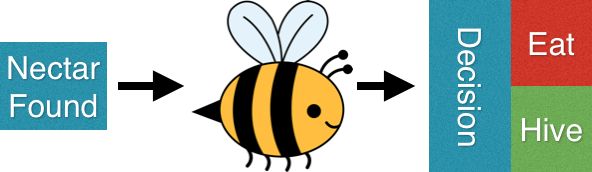
\includegraphics[height=3cm]{bee.png}
	\end{frame}

	\section{Hypothesis}
	\subsection{Outlooks}
	\begin{frame}{Dueling Outlooks}
		\begin{columns}[t]
			\column{.5\textwidth}

				\begin{block}{Alex the Pessimist}
						Neural nets insufficiently complicated for altruistic behavior to arise without considerable prompting.
				\end{block}

			\column{.5\textwidth}
				\begin{block}{Ravenna the Optimist}
		
						Agents will eventually figure out that the greatest benefit can be obtained through altruism.
					\begin{quote}
						``I want to believe!''
						\begin{flushright}
						 	-Ravenna
						\end{flushright} 
					\end{quote}
				\end{block}

		\end{columns}
	\end{frame}

	\subsection{Experimental Ideas}
	\begin{frame}{Most conducive environments to altruism}
		\begin{itemize}
			\item Incentivize altruism with explicitly higher fitness.
			\item Deincentivize selfishness with explicitly lower fitness.

			\item Some way of tying ``sharing'' fitness.
			\begin{itemize}
				\item The ``hive'' has an amount of honey to support the ``queen,'' and this influences fitness.
				\item Have all of the bees share the fitness of the hive.
				\item Have the health of the hive worked into the fitness function in another way
			\end{itemize}
		\end{itemize}
	\end{frame}


	\section{Demo}

	\subsection{Basic Experiments}

	\begin{frame}
		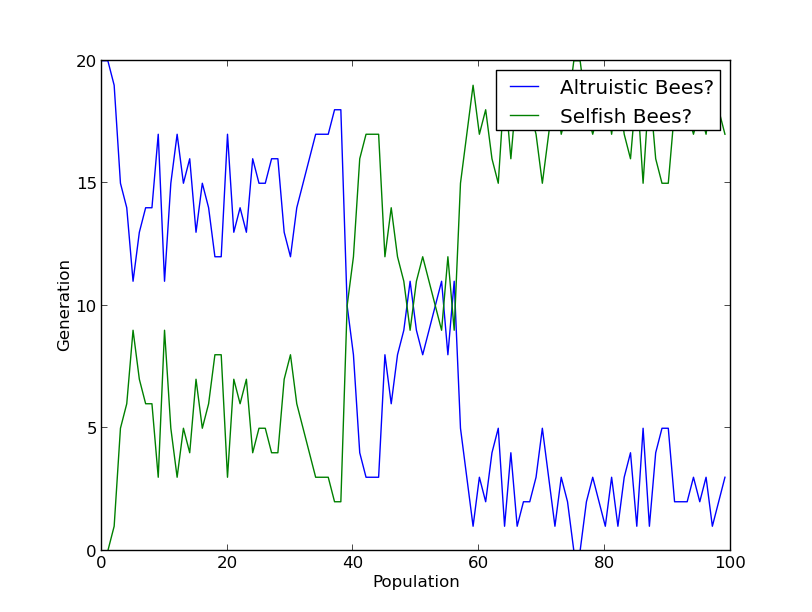
\includegraphics[width=7cm]{s_bees.png}
	\end{frame}

	\subsection{Hive-Based Fitness}

	\begin{frame}
		
	\end{frame}


	\subsection{Live Demo}
	\begin{frame}[fragile]{Live Demo}
		\begin{verbatim}
			python evolveHive.py
		\end{verbatim}
	\end{frame}

	\section{Q and A}
	\begin{frame}{Questions?}
		\titlepage
	\end{frame}

\end{document}